\textbf{Мотивация:}\\

Ранее мы рассматривали логистическую регрессию и log loss в виде логарифма от сигмоиды. Но данную задачу приближения loss function гладкой функцией можно решать и другими способами, один из них - SVM.\\

Давайте начнём с простого случая, когда у нас есть линейно разделимая выборка (хотя на практике такое вряд ли произойдет). Подумаем, как выбрать оптимальную гиперплоскость, которая разделяет два класса. Вопрос в том, что таких гиперплоскостей может быть очень много (например, какую-нибудь подходящую гиперплоскость можно чуть-чуть или даже не чуть-чуть пошевелить). \\

Получается, что много моделей представляют решение одной и той же задачи классификатора, и одно и то же значение эмпирического риска. В итоге у нас решение не единственно, а это плохо, потому что непонятно тогда, какое выбирать. \\

\begin{center}
    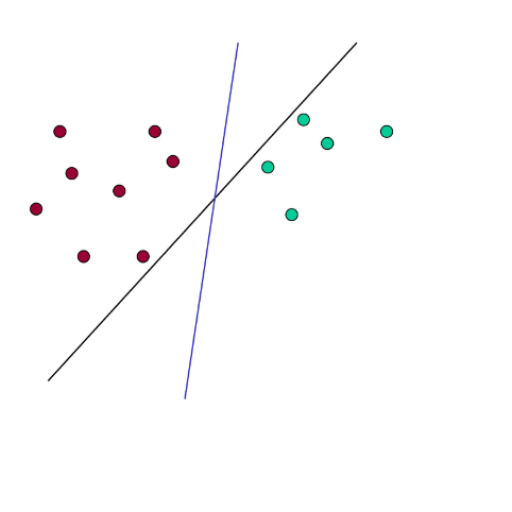
\includegraphics[scale=0.7]{images/11_1.png}
\end{center}

\textbf{Идея:}\\

Поэтому давайте поймем, какая модель (гиперплоскость) линейной классификации лучше? Полезно не только строить гиперплоскости, но и максимизировать ширину зазора между классами, которую эта гиперплоскость определяет (собственно, интуитивно кажется, что так разделение будет качественнее всего).

$$\exists w, w_0 : M_i(w, w_0) = y_i(\langle w, x_i \rangle - w_0) > 0 \forall i \in \{1, \dots, l\}$$

Формула выше представлена для ситуации, когда $bias$ не включен в вектор весов, и в вектор признаков не включена в начале $1$. Поэтому мы вычитаем ещё смещение $w_0$.

Если умножить гиперплоскость на константу, наклон не поменяется, поэтому мы можем произвести нормировку (никогда не было, и вот опять) $margin$ в $1$ с помощью изменения параметров модели $w$.

Раеммотрим следующую картинку: 

\begin{center}
    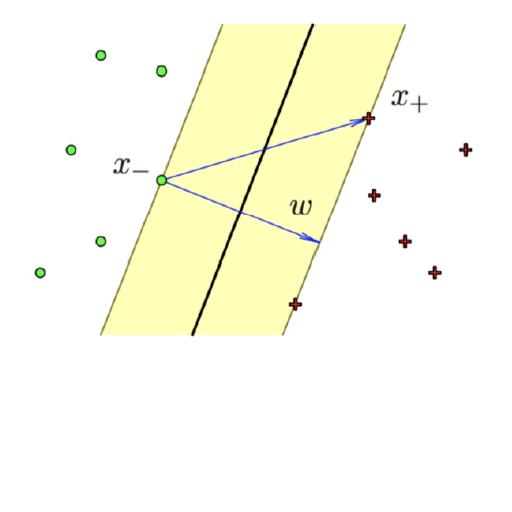
\includegraphics[scale=0.7]{images/11_2.png}
\end{center}

Отступ на ней это значение вектора $w_0$. Будем считать, что для самого левого красного плюсика (если смотреть на расстояние до гиперплоскости) у нас верно $\langle w, x_+ \rangle - w_0 = 1$. Тогда все точки правее будут иметь $\langle w, x \rangle - w_0 \geqslant 1$, а все точки левее самого правого зеленого кружочка будут
иметь $\langle w, x \rangle - w_0 \leqslant -1$. 

Мы хотим максимизировать ширину полосы между классами. Тогда давайте максимизировать, вспоминая линейную алгебру и то, как оценить расстояние от точки до прямой. Будем максимизировать расстояние между крайней левой точкой <<положительного>> класса, и крайней правой точкой <<отрицательного>> класса.

$$\frac{\langle x_+ - x_-, w \rangle}{\|w\|} \geqslant \frac{2}{\|w\|} \to \max$$

Широкая полоса между классами хороша тем, что даже имея девиации, классификатор всё ещё будет хорошо предсказывать разделение по классам. То есть если у нас появится в выборке несколько новых объектов, наш классификатор не будет резко менять свое решение, как могло произойти ранее. Потому что теперь мы не просто ищем гиперплоскость, но и максимизируем ширину между классами объектов.
Как мы уже сказали ранее, модуль отступа должен быть положителен для каждого класса объектов с учетом нашей нормировки, так как выборка линейно разделима по нашему предположению. Максимизируем модуль расстояния между классами, значит минимизируем квадратичный функционал нормы вектора весов:

$$ \begin{cases}
   \frac{1}{2}\|w\|^2 \to \min\limits_{w, w_0}\\
   M_i(w, w_0) \geqslant 1 & i = 1, \dots, l
 \end{cases}$$

Всё было бы здорово и задача оптимизации была бы поставлена, но мы сделали одно очень далекое от правды предположение, что наша выборка линейно разделима. На практике есть шум, сложные зависимости, которые не обязательно линейно разделяются. Или объекты одного класса могут попасть в глубину объектов другого класса (случайно попасть не в свою группу, а в другую). Как их разделять теперь, непонятно. И в этом случае у нас появляется отрицательный отступ, и все ломается.

Но есть выход. Можно просто ввести некоторый штраф за то, что объект попал к объектам другого класса.\\

\begin{center}
    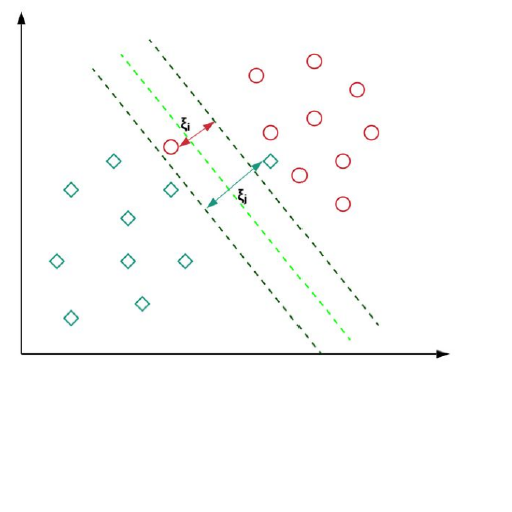
\includegraphics[scale=0.7]{images/11_3.png}
\end{center}

Новая постановка задачи будет выглядеть так (в ней $\xi_i$ как раз наш штрафной член):

$$\begin{cases}
   \frac{1}{2}\|w\|^2 + C\sum\limits_{i=1}^l \xi_i \to \min\limits_{w, w_0, \xi}\\
   M_i(w, w_0) \geqslant 1 - \xi_i & i = 1, \dots, l\\
   \xi_i \geqslant 0 & i = 1, \dots, l
 \end{cases}$$.

 Второе неравенство можем рассматривать как ограничение на $\xi_i$, если перенесем $\xi_i$ влево, а $margin$ вправо.

 Тогда, чтобы $\xi_i$ удовлетворяла обоим неравенствам (второму и третьему), нужно $\xi_i \geqslant \max(1 - M_i(w, w_0), 0)$.

 $C$ -- регуляризационная константа, которая отвечает за то, насколько сильно мы штрафуем модель.

 В итоге сумму, которую мы минимизируем, можно переписать как 

 $$C\sum\limits_{i=1}^l \max(0, 1- M_i(w, w_0)) + \frac{1}{2} \|w\|^2 \to \min\limits_{w, w_0}$$

 Правда, сейчас мы хоть и учли ограничения, но получили более сложную для решения задачу, ведь $\max(0, 1- M_i(w, w_0))$ не является гладкой функцией.\\

 Сейчас придется вспомнить методы оптимизации и теорему Каруша--Куна--Такера.

 В общем случае минимизация с заданными условиями это:

 $$\begin{cases}
   f(x) \to \min\limits_x\\
   g_i(x) \leqslant 0 & i = 1, \dots, m\\
   h_j(x) = 0 & j = 1, \dots, k
 \end{cases}$$

 Тогда у нас есть необходимые условия для локального минимума в общем случае:

 $$\begin{cases}
   \frac{\partial \mathcal{L}}{\partial w} = 0, \mathcal{L} = f(x) + \sum\limits_{i=1}^m \mu_ig_i(x) + \sum\limits_{j=1}^k \lambda_jh_j(x)\\
   g_i(x) \leqslant 0; h_j(x) = 0\\
   \mu_i(x) \geqslant 0\\
   \sum\mu_ig_i(x) = 0
 \end{cases}$$

 Можем расписать для нашего Лагранжиана:

 $$\mathcal{L}(w, w_0, \xi, \lambda, \eta) = \frac{1}{2}\|w\| - \sum\limits_{i=1}^{l} \lambda_i (M_i(w, w_0) - 1) - \sum\limits_{i=1}^{l}\xi_i (\lambda_i + \eta_i - C)$$

 Необходимые условия минимума:

 $$\begin{cases}
   \frac{\partial \mathcal{L}}{\partial w} = 0 \Rightarrow w = \sum\limits_{i=1}^l \lambda_i y_i x_i\\
   \frac{\partial \mathcal{L}}{\partial w_0} \Rightarrow \sum\limits_{i=1}^l \lambda_i y_i = 0\\
   \frac{\partial \mathcal{L}}{\partial \xi} = 0 \Rightarrow \eta_i + \lambda_i = C & i = 1, \dots, l\\
   \xi_i \geqslant 0, \lambda_i \geqslant 0, \eta_i \geqslant 0\\
   \lambda_i = 0 \vee M_i(w, w_0) = 1 - \xi_i\\
   \eta_i = 0 \vee \xi_i = 0
 \end{cases}$$

Так причём здесь метод опорных векторов (SVM)?
Делаем простое решение, в котором у нас участвуют только те объекты, которые так или иначе являются опорными объектами, то есть объектами, которые находятся около разделяющей полосы или внутри неё. Те объекты, которые лежат внутри своего класса, вообще говоря для нашего классификатора особо не играют роли, потому что та функция потерь, о которой мы говорим $\max(0, 1-M)$ реагирует только на те объекты, которые находятся внутри разделяющей полосы или в глубине чужого класса. 

Наша модель штрафуется не только в том случае, когда она неправильно проклассифицировала объект, но и за то, что они просто попали внутрь разделяющей полосы. 

\begin{center}
    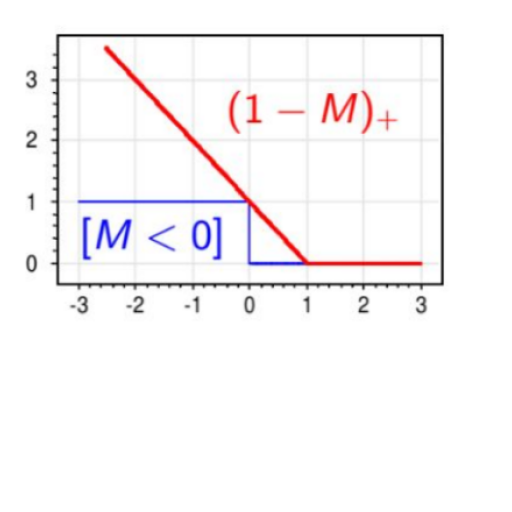
\includegraphics[scale=0.7]{images/11_4.png}
\end{center}

На картинке  наш настоящий лосс указан синей ступенькой, это тот лосс, который мы хотим минимизировать, а, значит, по рисунку видно, что тот функционал, который мы будем в итоге минимизировать, является верхней оценкой функции эмпирического риска. 

По сути, минимизируя красный функционал (Hinge loss), мы минимизируем mis loss.\\


\textbf{Теперь про регуляризацию}\\

Член функционала, состоящий из квадрата нормы вектора весов с некой константой - типичный регуляризационный член, от которого зависит ширина полосы. Напомним, что изначально мы хотели получить максимальную ширину полосы между классами. Мы пришли к привычному виду функции потерь:

$$Q(w, w_0) = \sum\limits_{i=1}^l[M_i(w, w_0) < 0] \leqslant \sum\limits_{i=1}^l \max(0, 1 - M_i(w, w_0)) + \frac{1}{2C}\|w\|^2 \to \min$$


Первое слагаемое отвечает за апроксмимацию решения, а второе - за регуляризацию. Константа $C$ в знаменателе регуляризационного члена появилась, потому что можно без нарушения общности поделить наш функционал на $C$ (заметим, что это та же $C$, что и в формулах ранее). 

Похожесть получившийся функции потерь на функцию потерь, например, в линейной регрессии, говорит нам о том, что есть общие подходы в математике построения моделей. И,  вообще говоря, добавление регуляризации привносит добавление некоего априорного знания внутрь нашей модели, в данном случае - максимизирует ширину межклассовой полосы. Так как константа стоит тут в знаменателе, то чем больше константа, тем слабее регуляризация и тем полоса уже. \\

\begin{center}
    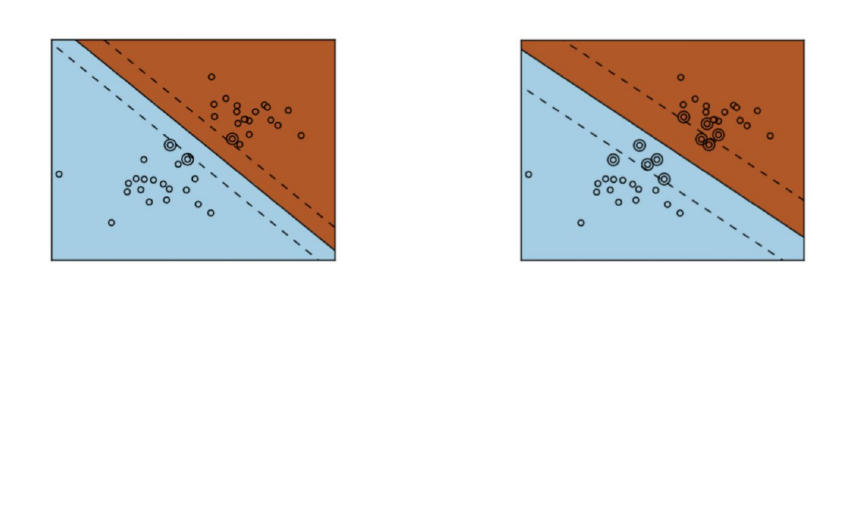
\includegraphics[scale=0.5]{images/11_5.png}
\end{center}

На этой картинке слева значение $C$ больше, справа -- меньше.

\textbf{Нелинейный SVM}\\

Внутри $margin$ лежит скалярное произведение. И, вообще говоря, мы можем использовать другое скалярное произведение, заданное для другого пространства.

Это основная идея нелинейного SVM: использовать другое преобразование для задания скалярного произведения на другом Гильбертовом пространстве. Для этого вводится функция ядра ($kernel$), которая обладает простыми свойствами. 

\begin{theorem}[теорема 1999 года Мерсера] функция может являться ядром, если она симметрична и неотрицательно определена,
$$K(x, x') : X \times X \to \R$$
$$\exists \phi : X \to H : \quad K(x, x') = \langle \phi(x), \phi(x') \rangle \text{, где } H \text{ --- шиьбертово пр-во}
$$
\end{theorem}

\begin{example}
Приведём несколько примеров ядер:

\begin{enumerate}
    \item $K(x, x') = \langle x, x' \rangle^2$
    \item $K(x, x') = \langle x, x' \rangle^d$
    \item $K(x, x') = (\langle x, x' \rangle + 1)^d$
    \item $K(x, x') = \exp((-\gamma\|x - x'\|^2)$ -- RBF
\end{enumerate}
\end{example}

\begin{center}
    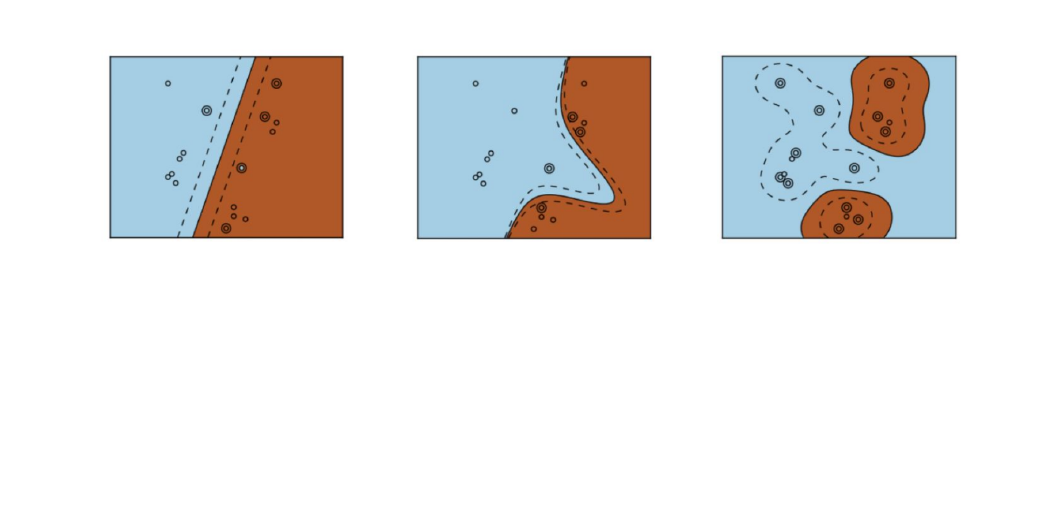
\includegraphics[scale=0.7]{images/11_6.png}
\end{center}

На картике слева разделяющая поверхность для скалярного произведения, по центру для полиномиального ядра, справа для $RBF$.

С различными ядрами мы можем строить различные разделяющие поверхности. Но проблема всё равно остаётся, популярность SVM упала за последние годы, так как чтобы подобрать ядро в таком алгоритме нужно перебрать возможные ядра, а возможные ядра подобрать <<экспертным мнением>>. Тем более если у нас много задач, в каждой из которых своя выборка, то каждый раз придётся проделывать одну и ту же работу. 

